\chapter{Título del Capítulo 2}
\label{ch:dos}

\noindent Los capítulos intermedios servían para cubrir los siguientes aspectos: antecedentes, problemática o estado del arte, objetivos, fases y desarrollo del proyecto.

En el capítulo anterior se ha introducido la \autoref{fig:intro} y en este la \autoref{fig:other}. 

\section{Primera sección de otro capítulo}
\label{sec:ch2_1}

\begin{figure}[htbp]
   \centering
   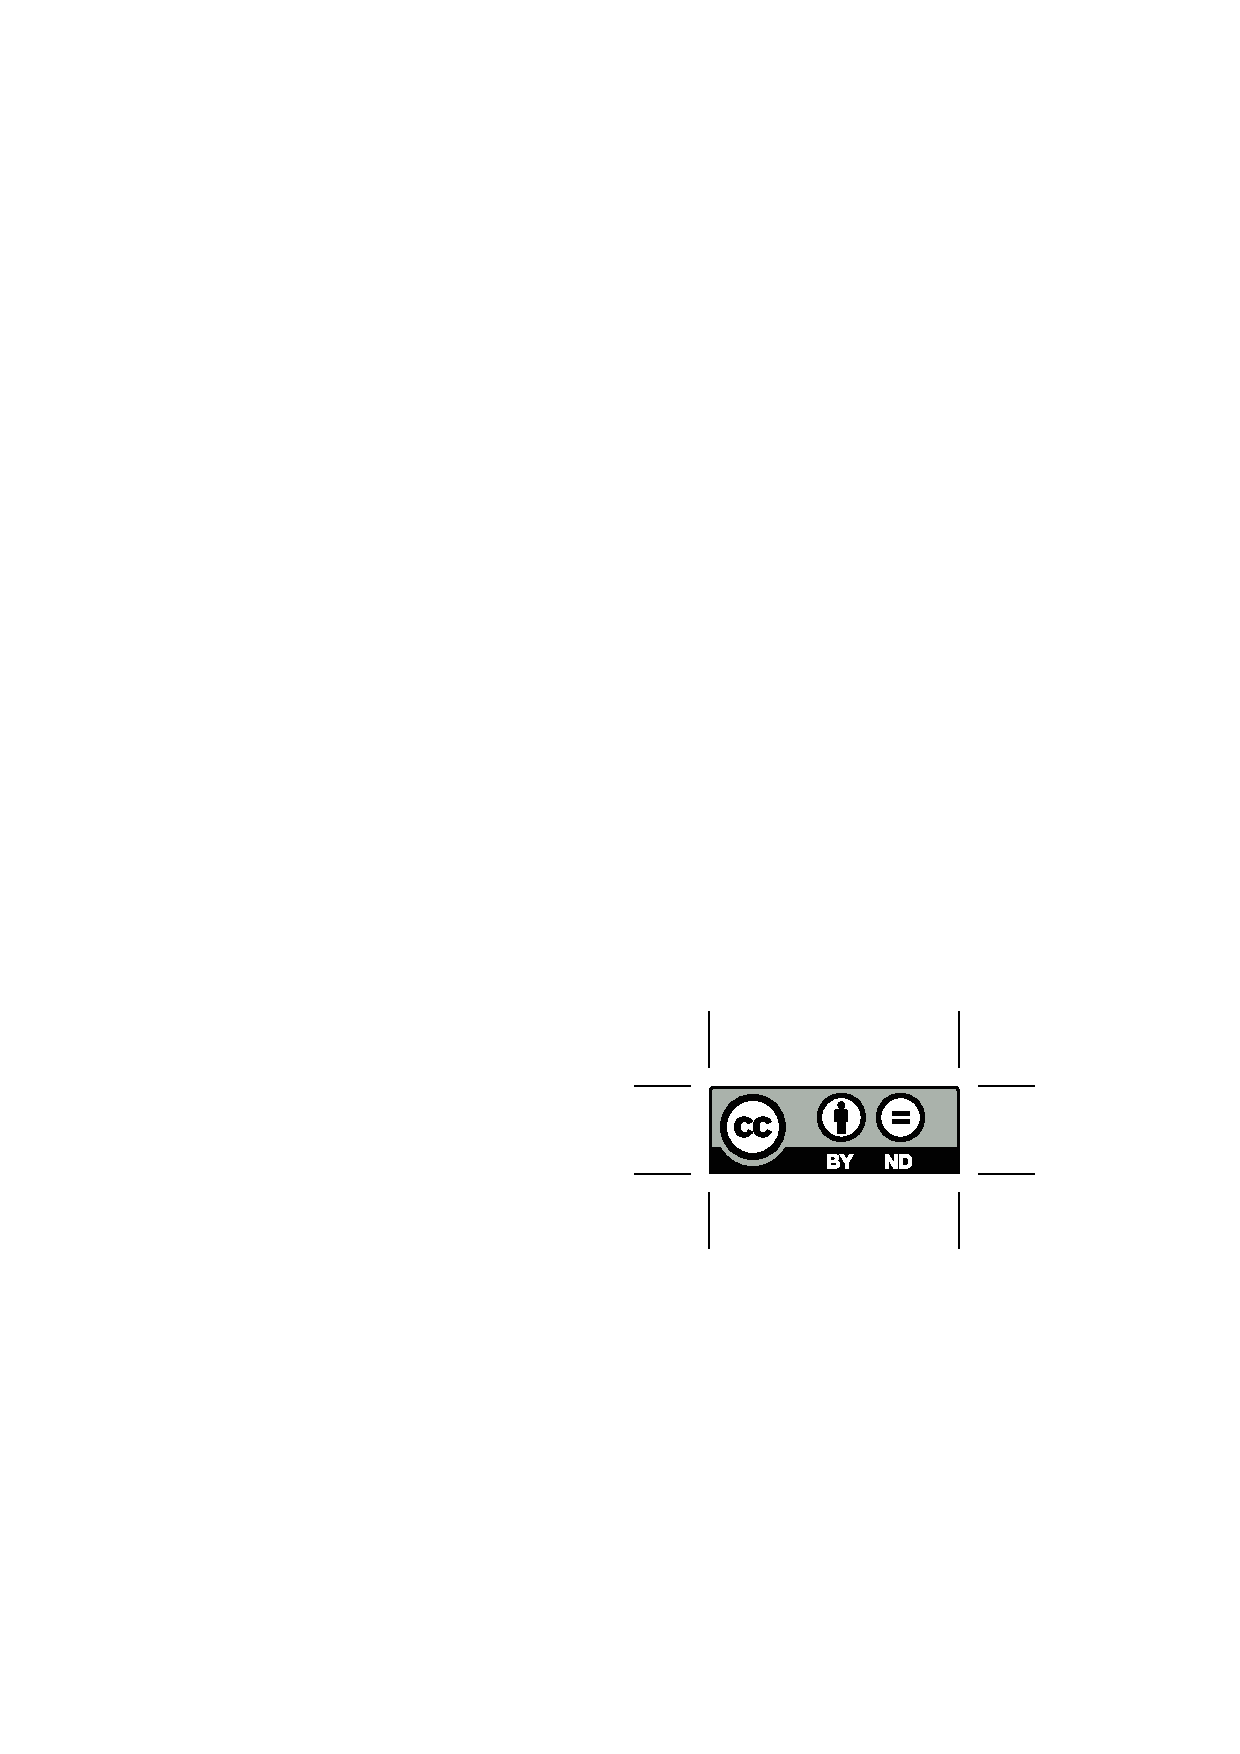
\includegraphics[width=0.5\linewidth]{images/licenses/by-nd}
   \caption{Otra figura.}
   \label{fig:other}
\end{figure}

\lipsum[3]

\section{Segunda sección de otro capítulo}

\noindent \lipsum[4-5]


